\documentclass[../../main.tex]{subfiles}
\begin{document}

{\bf [解]}
$a_n$個の円の中心を$O_1\sim O_n$，半径1の円の中心を$O$とする．
円をできる限り多く外接させるためには$a_n$個の円をお互いが接するように配置していけば良いから，以下この場合を考える．（ただし，$O_1$と$O_n$は接するとは限らない．）
この時円$O_i, O_{i+1}$の接点を$H_i$とおく．
図のように外接円の半径が作る角度（または$O_1, O_2$の作る角度の半分）を$\theta$とおく：
\begin{align}
 \angle O_1H_1O_2 = \theta \label{eq:1}
\end{align}

\begin{figure}[htb]
\begin{center}
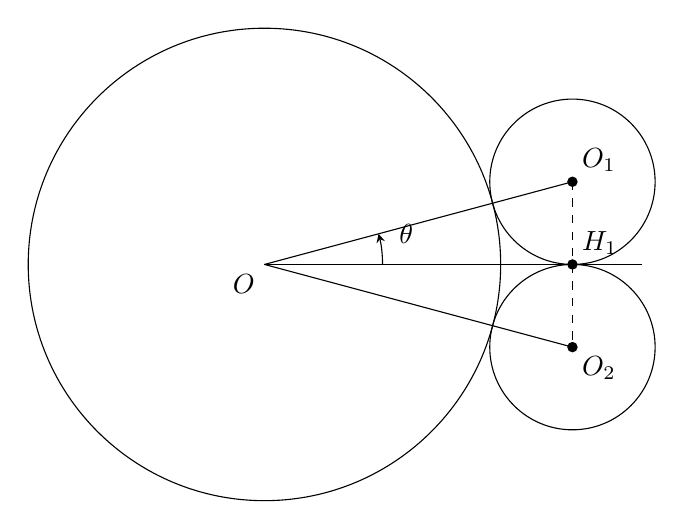
\begin{tikzpicture}[scale=3, >=stealth]
  % 半径1の円 (O_1,O_2 の図示用に小円の半径は 0.35 とやや誇張して図示)
  \draw (0,0) circle (1);
  \node[below left] at (0,0) {$O$};
  % 基準線 (O_1,O_2 を結ぶ接点方向: 角の二等分線)
  \draw (0,0) -- (1.6,0);
  % 角 theta (sin theta = 0.35/1.35 の二等分線からの角)
  \draw[->] (0.5,0) arc (0:15.03:0.5);
  \node[right] at (0.53,0.13) {$\theta$};
  \draw (0,0) -- (1.30384,0.35);
  \draw (0,0) -- (1.30384,-0.35);
  \draw[dashed] (1.30384,0.35) -- (1.30384,-0.35);
  \fill (1.30384,0.35) circle (0.63pt);
  \fill (1.30384,-0.35) circle (0.63pt);
  \fill (1.30384,0) circle (0.63pt);
  \draw (1.30384,0.35) circle (0.35);
  \draw (1.30384,-0.35) circle (0.35);
  \node[above right] at (1.30384,0.35) {$O_1$};
  \node[below right] at (1.30384,-0.35) {$O_2$};
  \node[above right] at (1.30384,0.0) {$H_1$};
\end{tikzpicture}
\end{center}
\caption{円の配置と角$\theta$}
\end{figure}

この時図より
\begin{align}
\sin\theta=\dfrac{O_1H}{OO_1} = \dfrac{\dfrac{1}{n}}{1+\dfrac{1}{n}}=\dfrac{1}{n+1} \quad \cdots \text{①} \label{eq:2}
\end{align}
と計算できる．

題意より$a_n$個の円を並べた時にお互いが重ならず，かつ追加の円も配置できないから
\begin{align}
2a_n\cdot\theta&\le2\pi<2(a_n+1)\theta \\
\therefore 
\dfrac{\pi}{n\theta}-\dfrac{1}{n}&\le\dfrac{a_n}{n}<\dfrac{\pi}{n\theta} \quad \cdots \text{②}\ (\because n>0) \label{eq:3}
\end{align}
である．

ここで\cref{eq:2}より$n\to\infty$の時$\theta\to 0$である．これと\cref{eq:2}から
\begin{align}
\dfrac{1}{n\theta}=\dfrac{1}{n\sin\theta}\cdot\dfrac{\sin\theta}{\theta}=\dfrac{n+1}{n}\cdot\dfrac{\sin\theta}{\theta}=\dfrac{1+\dfrac{1}{n}}{1}\cdot\dfrac{\sin\theta}{\theta}\longrightarrow 1 \quad(n\to\infty)
\end{align}
である．
よって\cref{eq:3}と挟み撃ちの定理より
\begin{align}
\lim_{n\to\infty}\dfrac{a_n}{n} = \pi
\end{align}
である．


\newpage

\end{document}
